\documentclass[12pt]{extarticle}
\usepackage{extsizes}
\usepackage{xcolor}
\usepackage{amsmath}
\usepackage{tikz}
\usepackage{graphicx}
\usepackage{fancyhdr}
\usepackage[paperwidth=210mm, paperheight=250mm, vmargin=2cm, hmargin=1.5cm]{geometry}

\pagestyle{fancy}
\fancyhf{}
\lhead{The Length of an Arc}
\rhead{Page \thepage}
\renewcommand{\headrulewidth}{0.4pt} % Add this line

\makeatletter
\renewcommand{\maketitle}{
  \begin{center}
    {\Huge \@title}
    \vspace{0cm} % Adjust this value to change the space after the title
  \end{center}
}
\makeatother

\title{The Length of an Arc}
\begin{document}
\thispagestyle{empty}
\maketitle



\hrulefill

\section{Introduction}
Many times when solving problems it is useful to know the length of a curve. By the end of this lesson we will be able to find the lengths of curves using integrals and derivatives!

\section{Derivation for functions}

We already know how to calculate the length of a straight line using the Pythagorean theorem
\begin{equation}
    \text{Length of a straight line} = \sqrt{(x_2 - x_1)^2 + (y_2 - y_1)^2}
\end{equation}

We can first start by splitting our curve into many small straight line segments segments of width $\Delta x$

The sum of all these line segments (as $\Delta x$ goes to zero) approaches the length of the line 

\begin{align}
    \sum \sqrt{{\Delta x}^2 + {\Delta y}^2}
\end{align}

\begin{center}
    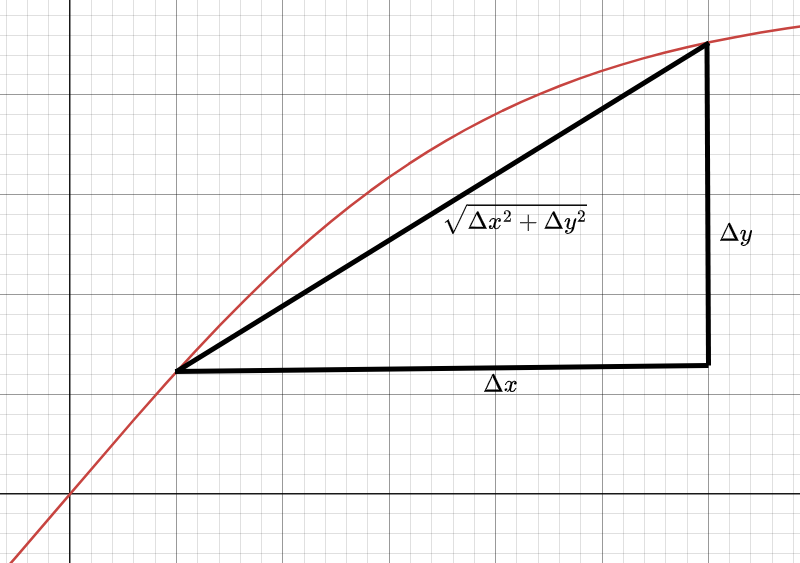
\includegraphics[height = 0.4\textheight]{proofImage1.png}
\end{center}

So now we have to find a way to write this where we can evaluate a riemann sum (and thus an integral).
We can factor out $\Delta x^2$ from both deltas inside the equation

\begin{align}   
    \sum \sqrt{{\Delta x^2}(1 + {(\frac{\Delta y}{\Delta x}})^2)} \\
    \sum \sqrt{(1 + {(\frac{\Delta y}{\Delta x}})^2)} \cdot \Delta x
\end{align}

As $\Delta x$ approaches 0, we realize this is a riemann sum and can use the fundamental theorem of calculus to evalute it 
We also see that $\frac{\Delta x}{\Delta y}$ is the derivative of the function, so we can replace it in our formula

\begin{align}
    \text{Length of a curve} &= \int_{a}^{b} \sqrt{1 + f'(x)^2} \cdot dx
\end{align}

\section{Practice}
\textbf{Example 1.} Find the arc length of a unit semicircle (since we know the formula for the perimeter of a circle we know our answer should be $\frac{2\pi (1)}{2} = \pi$)
\begin{align}
    f(x) &= \sqrt{1-x^2} \\
    \text{Arc length} &= \int_{-1}^{1} \sqrt{1 + f'(x)^2} dx 
\end{align}

\begin{center}
\begin{tikzpicture}
    \draw[step = 0.5cm, gray, very thin] (-1.5,-1.5) grid (1.5,1.5);
    \draw (-1,0) arc (180:0:1cm);
\end{tikzpicture}
\end{center}

\vspace{10cm}


\textbf{Example 2.} Find the arc length of $\log(\sec(x))$ from $-\frac{\pi}{4}$ to $\frac{\pi}{4}$

\vspace{10cm}

\textbf{Example 3.} Find the surface area length of strip $y = x^{3/2} $ from $x = 0$ to $x= 4$, when stretched across the z-axis by 4 units

\begin{center}
    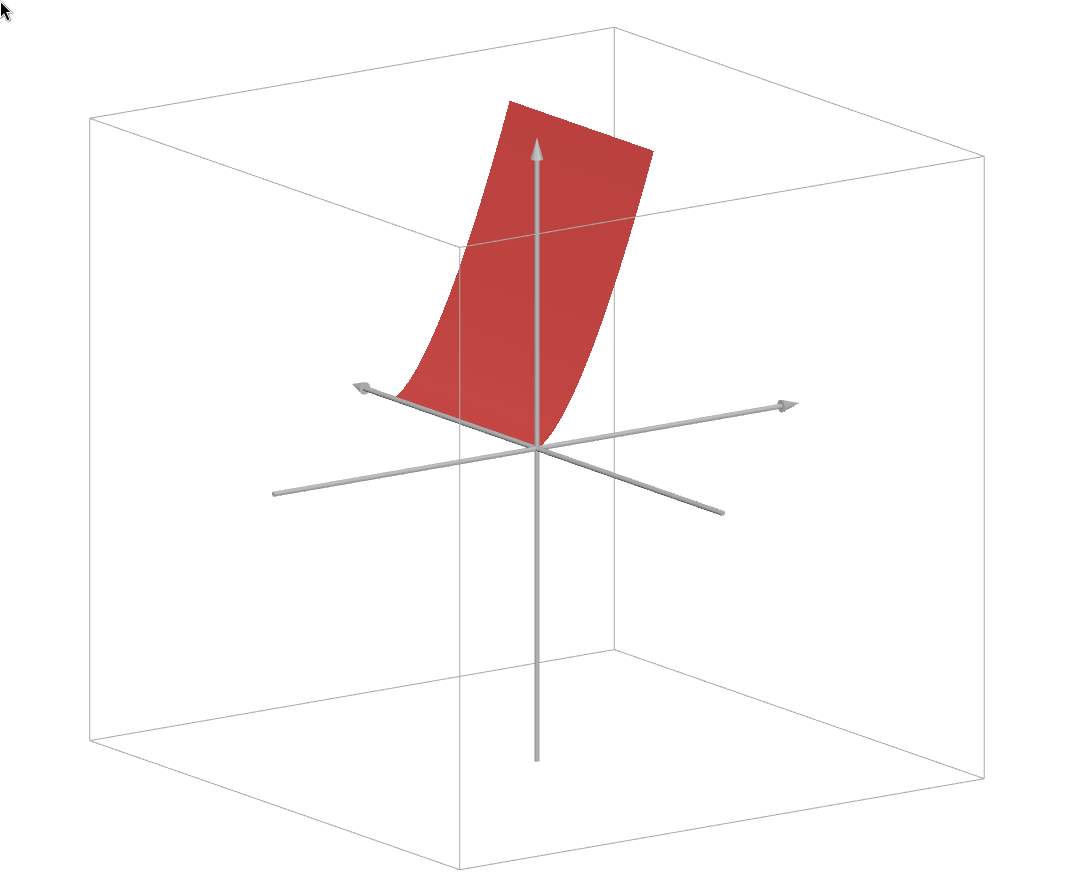
\includegraphics[height = 0.2\textwidth]{Surface.png}
\end{center}

\vspace{10cm}

\section{Arc Length of Parametric Functions}

For the derivation of the arc length of parametric functions, we will go a slightly different route \\
We will be using the derivative of both the $x$ component and the $y$ component \\ We know the our change in $y$ can be found by using the parametric equation for $y$ based on $t$, and the same thing can be said for the change in $x$

\begin{align} 
    \text{Change in y} &= \Delta y = \frac{\Delta y}{\Delta t} \cdot \Delta t \\
    \text{Change in x} &= \Delta x = \frac{\Delta x}{\Delta t} \cdot \Delta t  
\end{align}

Now lets use our initial formula again to find the arc length of a parametric function


\begin{align} 
    &= \sum \sqrt{(\frac{\Delta x}{\Delta t} \cdot \Delta x)^2 + (\frac{\Delta y}{\Delta t} \cdot \Delta t) ^ 2} \\ 
    &= \sum \sqrt{(\Delta t)^2((\frac{\Delta x}{\Delta t})^2 + (\frac{\Delta y}{\Delta t}) ^ 2)} \\ 
    &= \sum \sqrt{(\frac{\Delta x}{\Delta t})^2 + (\frac{\Delta y}{\Delta t}) ^ 2} \cdot \Delta t \\ 
\end{align}

And treating this as a riemann sum we can then use integral calculus to evaluate as $\Delta t$ goes to zero and this leaves us with the following formula for the arc length of a parametric function:

\begin{align} 
    \text{Length of a parametric curve} &= \int_{a}^{b} \sqrt{(\frac{dx}{dt})^2 + (\frac{dy}{dt}) ^ 2} \cdot dt  
\end{align}

\section{Finding lengths of parametric functions}

\textbf{Example 1.} Lets revisit our first example, finding the length of half an arc of a unit circle (from $0$ to $\pi$), since we can now rewrite it using the following parametric functions
\begin{align} 
    x = \sin(t) \\ 
    y = \cos(t) 
\end{align}

\vspace{10cm}

\textbf{Example 2.} Find the length of the following parametric curve from $t = -2$ to $t = 2$

\begin{align} 
    x &= t^3 - 3t \\ 
    y &= 3t^2  
\end{align}

\begin{center}
    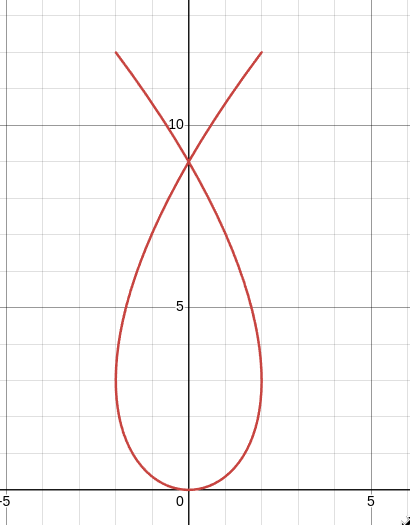
\includegraphics[height = 0.3\textheight]{Graph.png}
\end{center}

\vspace{10cm}

\end{document}